% \begin{figure*}[t]
%   \centering
%   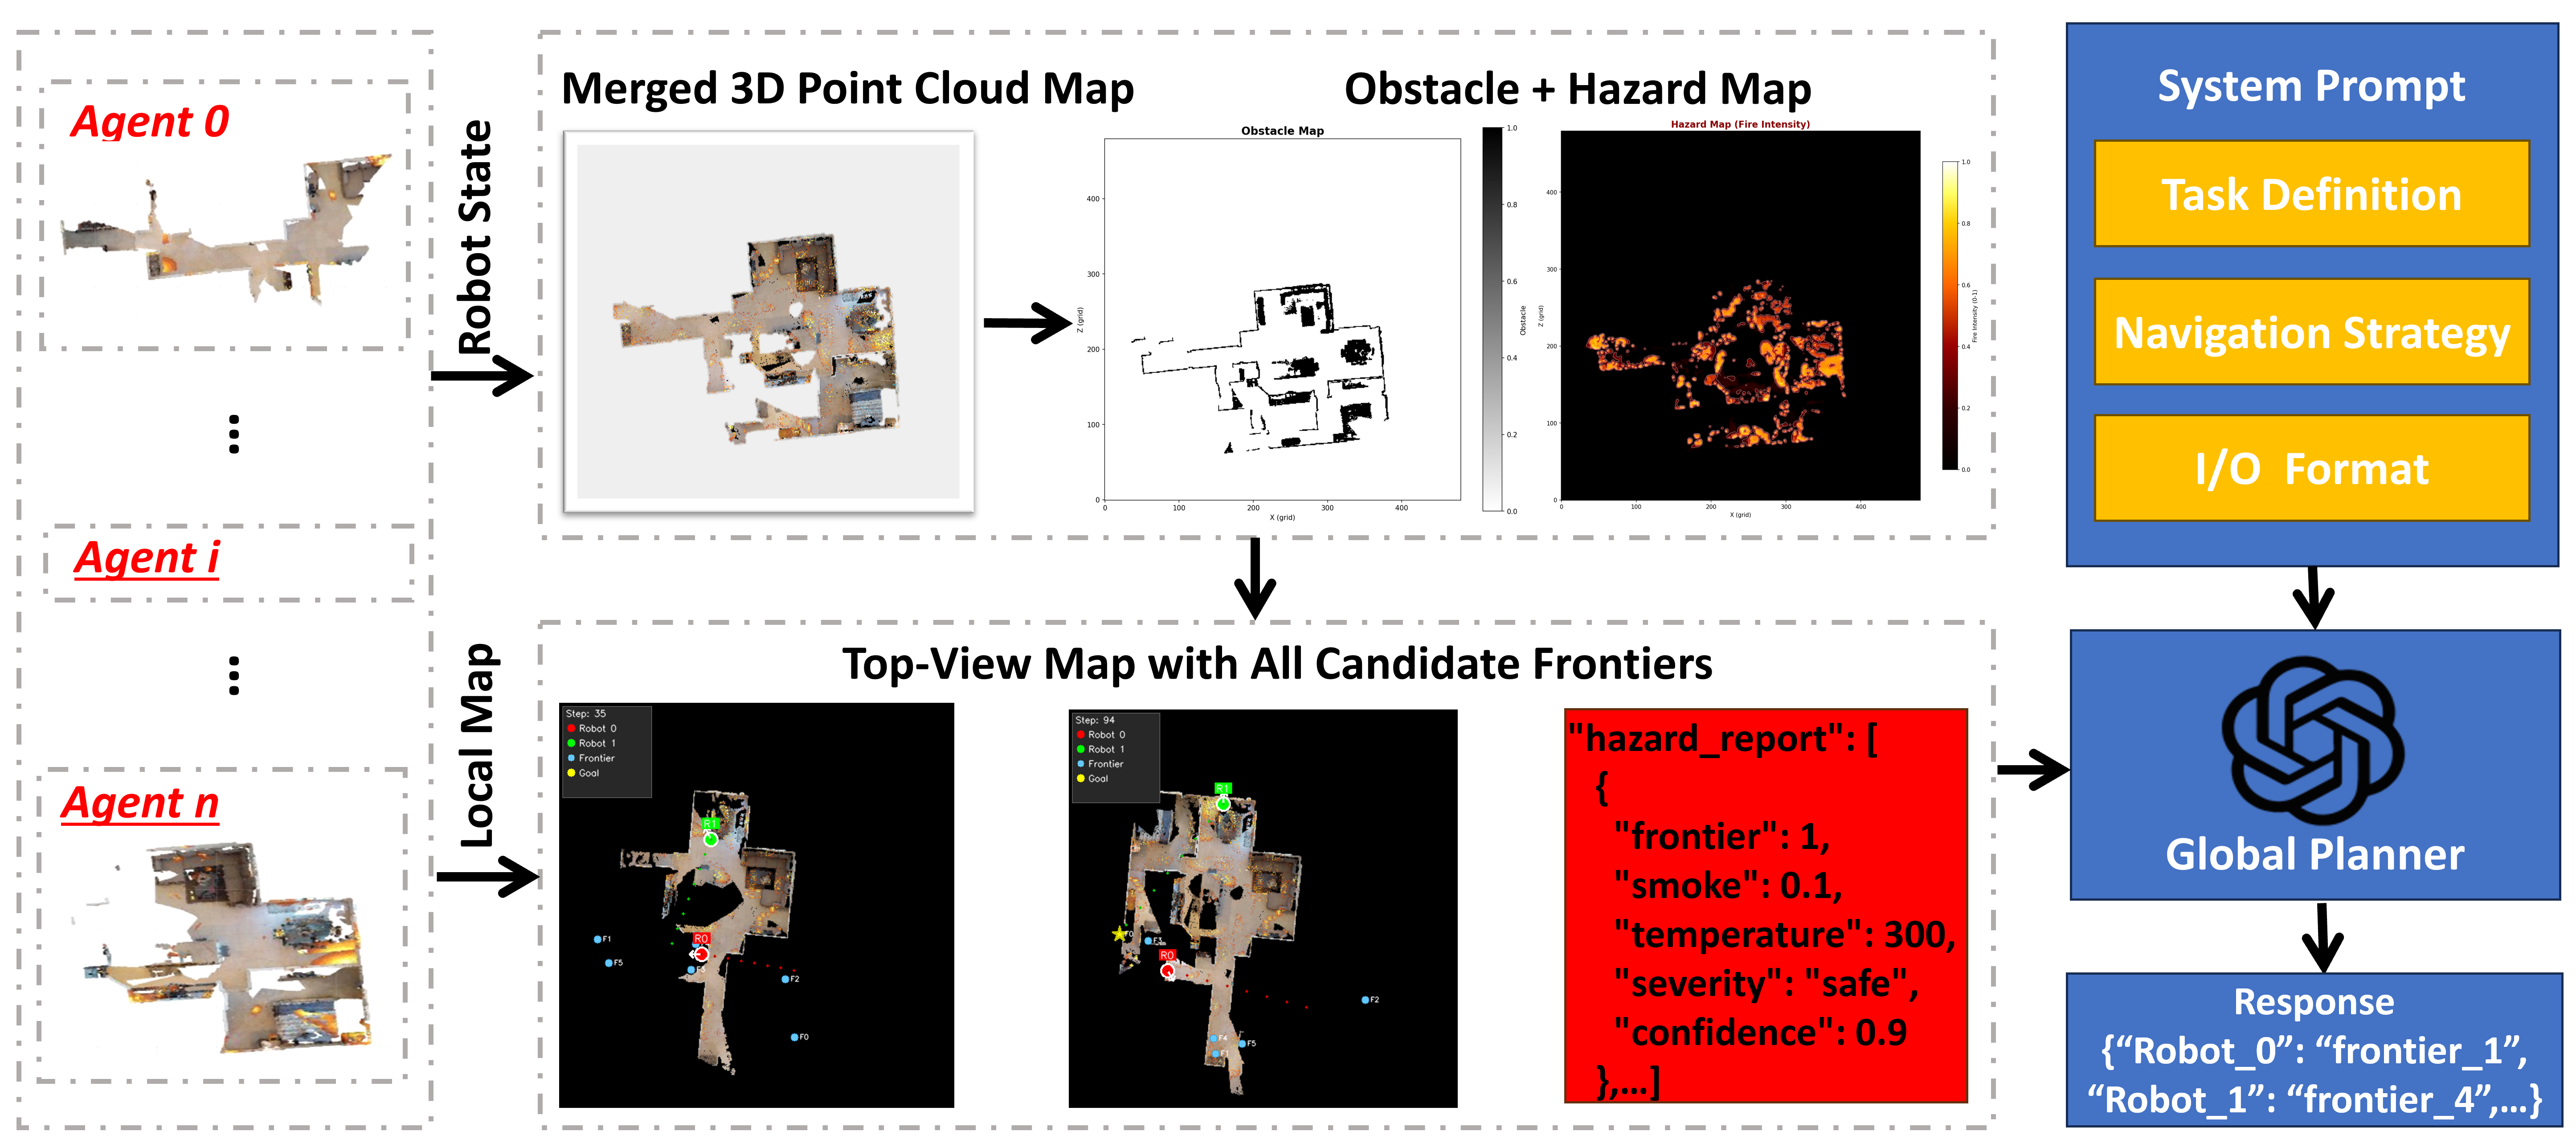
\includegraphics[width=\textwidth]{figures/Cooerative Navigation using llm.png}
%   \caption{structure.}
%   \label{fig:overview}
% \end{figure*}


% \subsection{Task Definition}

% We consider a \emph{multi-agent cooperative SAR} task in fire driven indoor environments, where a team of mobile robots collaboratively explores an unknown scene to locate victims or mission critical target objects under hazardous conditions. Let $\mathcal{C} = \{c_1, \ldots, c_m\}$ denote the set of target categories (e.g., \emph{human}, \emph{fire extinguisher}, \emph{bathroom}), and let $\mathcal{S} = \{s_1, \ldots, s_K\}$ denote the set of indoor scenes affected by fire, smoke, and structural damage.

% For each episode, a team of $N$ robots $\mathcal{R} = \{r_1, \ldots, r_N\}$ is deployed in a scene $s_i \in \mathcal{S}$. All robots are initialized at a common starting location $\mathbf{p}_i$, but with different initial orientations to reflect realistic deployment constraints in emergency response. Each robot is assigned the same target category $c_i \in \mathcal{C}$. An episode is therefore defined as:
% \begin{equation}
% \mathcal{T}_i = \{N, s_i, c_i, \mathbf{p}_i\}.
% \end{equation}

% The observation space $\mathcal{O}$ consists of four main modalities: RGB images, depth images, thermal images, and mmWave radar reflected signals, which jointly provide complementary visual, geometric, and smoke-robust perception information. The action space $\mathcal{A}$ consists of six discrete actions:
% \{\texttt{move\_forward}, \texttt{turn\_left}, \texttt{turn\_right}, \texttt{look\_up}, \texttt{look\_down}, \texttt{stop}\}, where \texttt{move\_forward} action advances the robot by $0.25\,\text{m}$, while the rotational actions, including \texttt{turn\_left}, \texttt{turn\_right}, \texttt{look\_up}, and \texttt{look\_down}, rotate the robot by $30^{\circ}$ in the corresponding direction.

% At each discrete time step $t$, each robot $r_i$ receives a
% multi-modal observation $o_t^i \in \mathcal{O}$ from its local perspective and simultaneously executes a single action $a_t^i$ from $\mathcal{A}$. % The \texttt{stop} action is triggered when a robot determines that it has reached the specific number of goal objects or explored the entire map. 
% An episode is considered successful if the team of agents safely reaches the specified number of target instances of category \(c_i\) within a distance threshold of \(0.1\,\text{m}\) or explores the entire environment while all agents remain within survivable hazard limits throughout the episode.
\subsection{Task Definition}
We consider a \emph{multi-agent cooperative SAR} task in fire-driven indoor environments, where a team of mobile robots explores an unknown scene to locate victims or mission-critical targets under hazardous conditions. Let $\mathcal{C} = \{c_1, \ldots, c_m\}$ denote the set of target categories (e.g., \emph{human}, \emph{fire extinguisher}, \emph{bathroom}), and let $\mathcal{S} = \{s_1, \ldots, s_K\}$ denote the set of fire-affected indoor scenes. In each episode, $N$ robots $\mathcal{R} = \{r_1, \ldots, r_N\}$ are deployed in a scene $s_i \in \mathcal{S}$ from a shared starting position $\mathbf{p}_i$ with different initial orientations to reflect realistic emergency deployment. All robots are assigned the same target category $c_i \in \mathcal{C}$. The episode is defined as:
\begin{equation}
\mathcal{T}_i = \{N, s_i, c_i, \mathbf{p}_i\}.
\end{equation}

The observation space $\mathcal{O}$ comprises four modalities: RGB, depth, thermal imaging, and mmWave radar, providing complementary visual, geometric, and smoke-robust perception. The action space $\mathcal{A}$ consists of six discrete actions:
\{\texttt{move\_forward}, \texttt{turn\_left}, \texttt{turn\_right}, \texttt{look\_up}, \texttt{look\_down}, \texttt{stop}\}. The \texttt{move\_forward} action advances the robot by $0.25\,\text{m}$, and each rotational action changes orientation by $30^{\circ}$. At each discrete time step $t$, robot $r_i$ receives a multi-modal observation $o_t^i \in \mathcal{O}$ and executes an action $a_t^i \in \mathcal{A}$. An episode is successful if the team reaches the required number of target instances of category $c_i$ within a $0.1\,\text{m}$ distance threshold, or fully explores the environment, while all agents remain within survivable hazard limits throughout the episode.


% Each agent is allowed a maximum of $T_{\max}=500$ time steps per episode. The collective objective of the agent team is to minimize exploration time and cumulative hazard exposure, while maximizing spatial coverage and overall task success rate, under dynamic and adverse conditions characterized by fire propagation, smoke-induced visibility degradation, and unreliable sensing.
\subsection{Overview}
As illustrated in Fig.~\ref{fig:System Design}, we propose a hazard-aware multi-agent navigation framework, \system, tailored for indoor fire SAR scenarios. Each agent performs robust multi-modal perception by jointly fusing RGB-D, thermal imaging, and mmWave radar to see through smoke and construct a local hazard-annotated 3D point cloud encoding geometry, temperature, smoke and sensing uncertainty. These local maps are merged into a global representation, which is further projected into a compact 2D obstacle and hazard map for frontier extraction and risk assessment. Leveraging this structured spatial and hazard-aware abstraction, a VLM serves as a global planner, reasoning jointly over robot states, frontier utility, and environmental risks to assign safe and efficient exploration goals to each agent. Finally, a hazard-aware Fast Marching Method (FMM) local planner refines these assignments into collision-free and risk-sensitive trajectories. Together, this hierarchical design enables coordinated, safe, and efficient multi-agent exploration under dynamic, fire-driven indoor conditions.

\subsection{Multi-modal Perception and Fusion}
To maintain reliable situational awareness under such harsh conditions, our framework adopts a robust multi-modal perception pipeline that integrates RGBD, thermal imaging, and mmWave radar signals as illustrated in Fig.~\ref{fig:multi_modal_perception_and_fusion}. The goal is to (1) extract stable structural cues, (2) detect fire-related hazards, and (3) produce a unified hazard-aware map for downstream planning.

For each robot $r_i$, given a sequence of synchronized multi-modal observations collected in indoor fire environments,
including RGB, depth, and thermal images,
\begin{equation}
\mathcal{I}_i =
\left\{
\left(I^{i}_{1,\mathrm{rgb}}, I^{i}_{1,\mathrm{d}}, I^{i}_{1,\mathrm{th}}\right), \dots,
\left(I^{i}_{t,\mathrm{rgb}}, I^{i}_{t,\mathrm{d}}, I^{i}_{t,\mathrm{th}}\right)
\right\},
\end{equation}
and the corresponding mmWave radar observations and the associated robot poses are:
\begin{equation}
\mathcal{M}_i^{\mathrm{rad}} =
\left\{
m_1^i, \dots, m_t^i
\right\}, \quad
\mathcal{P}_i = \{p^i_1, \dots, p^i_t\}.
\end{equation}
Each robot incrementally constructs a local hazard-aware 3D point cloud map $\mathcal{M}_i$ through the multi-modal perception and its pose.
% In indoor fire scenarios, visual perception is severely degraded by dense smoke, dynamic flames, and extreme illumination conditions,
% leading to significant loss of structural details in RGB images and increased noise or missing values in depth measurements.
% To address this challenge, we perform a high-level multi-modal fusion that integrates RGB, depth, and thermal observations to recover a
% \emph{see-through-smoke} visual representation.

Specifically, at each time step $t$, three visual modalities are first spatially and temporally aligned.
The aligned observations are then jointly processed by a VLM-based fusion operator $\mathcal{F}_{\mathrm{vlm}}(\cdot)$ to infer an enhanced visual representation:
\begin{equation}
I^{i}_{t,\mathrm{fused}} =
\mathcal{F}_{\mathrm{vlm}}
\left(
I^{i}_{t,\mathrm{rgb}},
I^{i}_{t,\mathrm{d}},
I^{i}_{t,\mathrm{th}}
\right).
\end{equation}
% where $\mathcal{F}_{\mathrm{vlm}}(\cdot)$ denotes a semantic-aware multi-modal fusion operator that leverages both visual cues and learned cross-modal priors.
% By reasoning over these complementary modalities, the VLM infers a visually enhanced representation that restores occluded structures,
% suppresses smoke-induced artifacts, and preserves scene semantics.
The resulting fused image $I^{i}_{t,\mathrm{fused}}$ approximates a \emph{smoke-transparent} view of the environment, enabling more reliable downstream tasks such as 3D reconstruction, hazard mapping, and frontier extraction.

\begin{figure}[t]
  \centering
  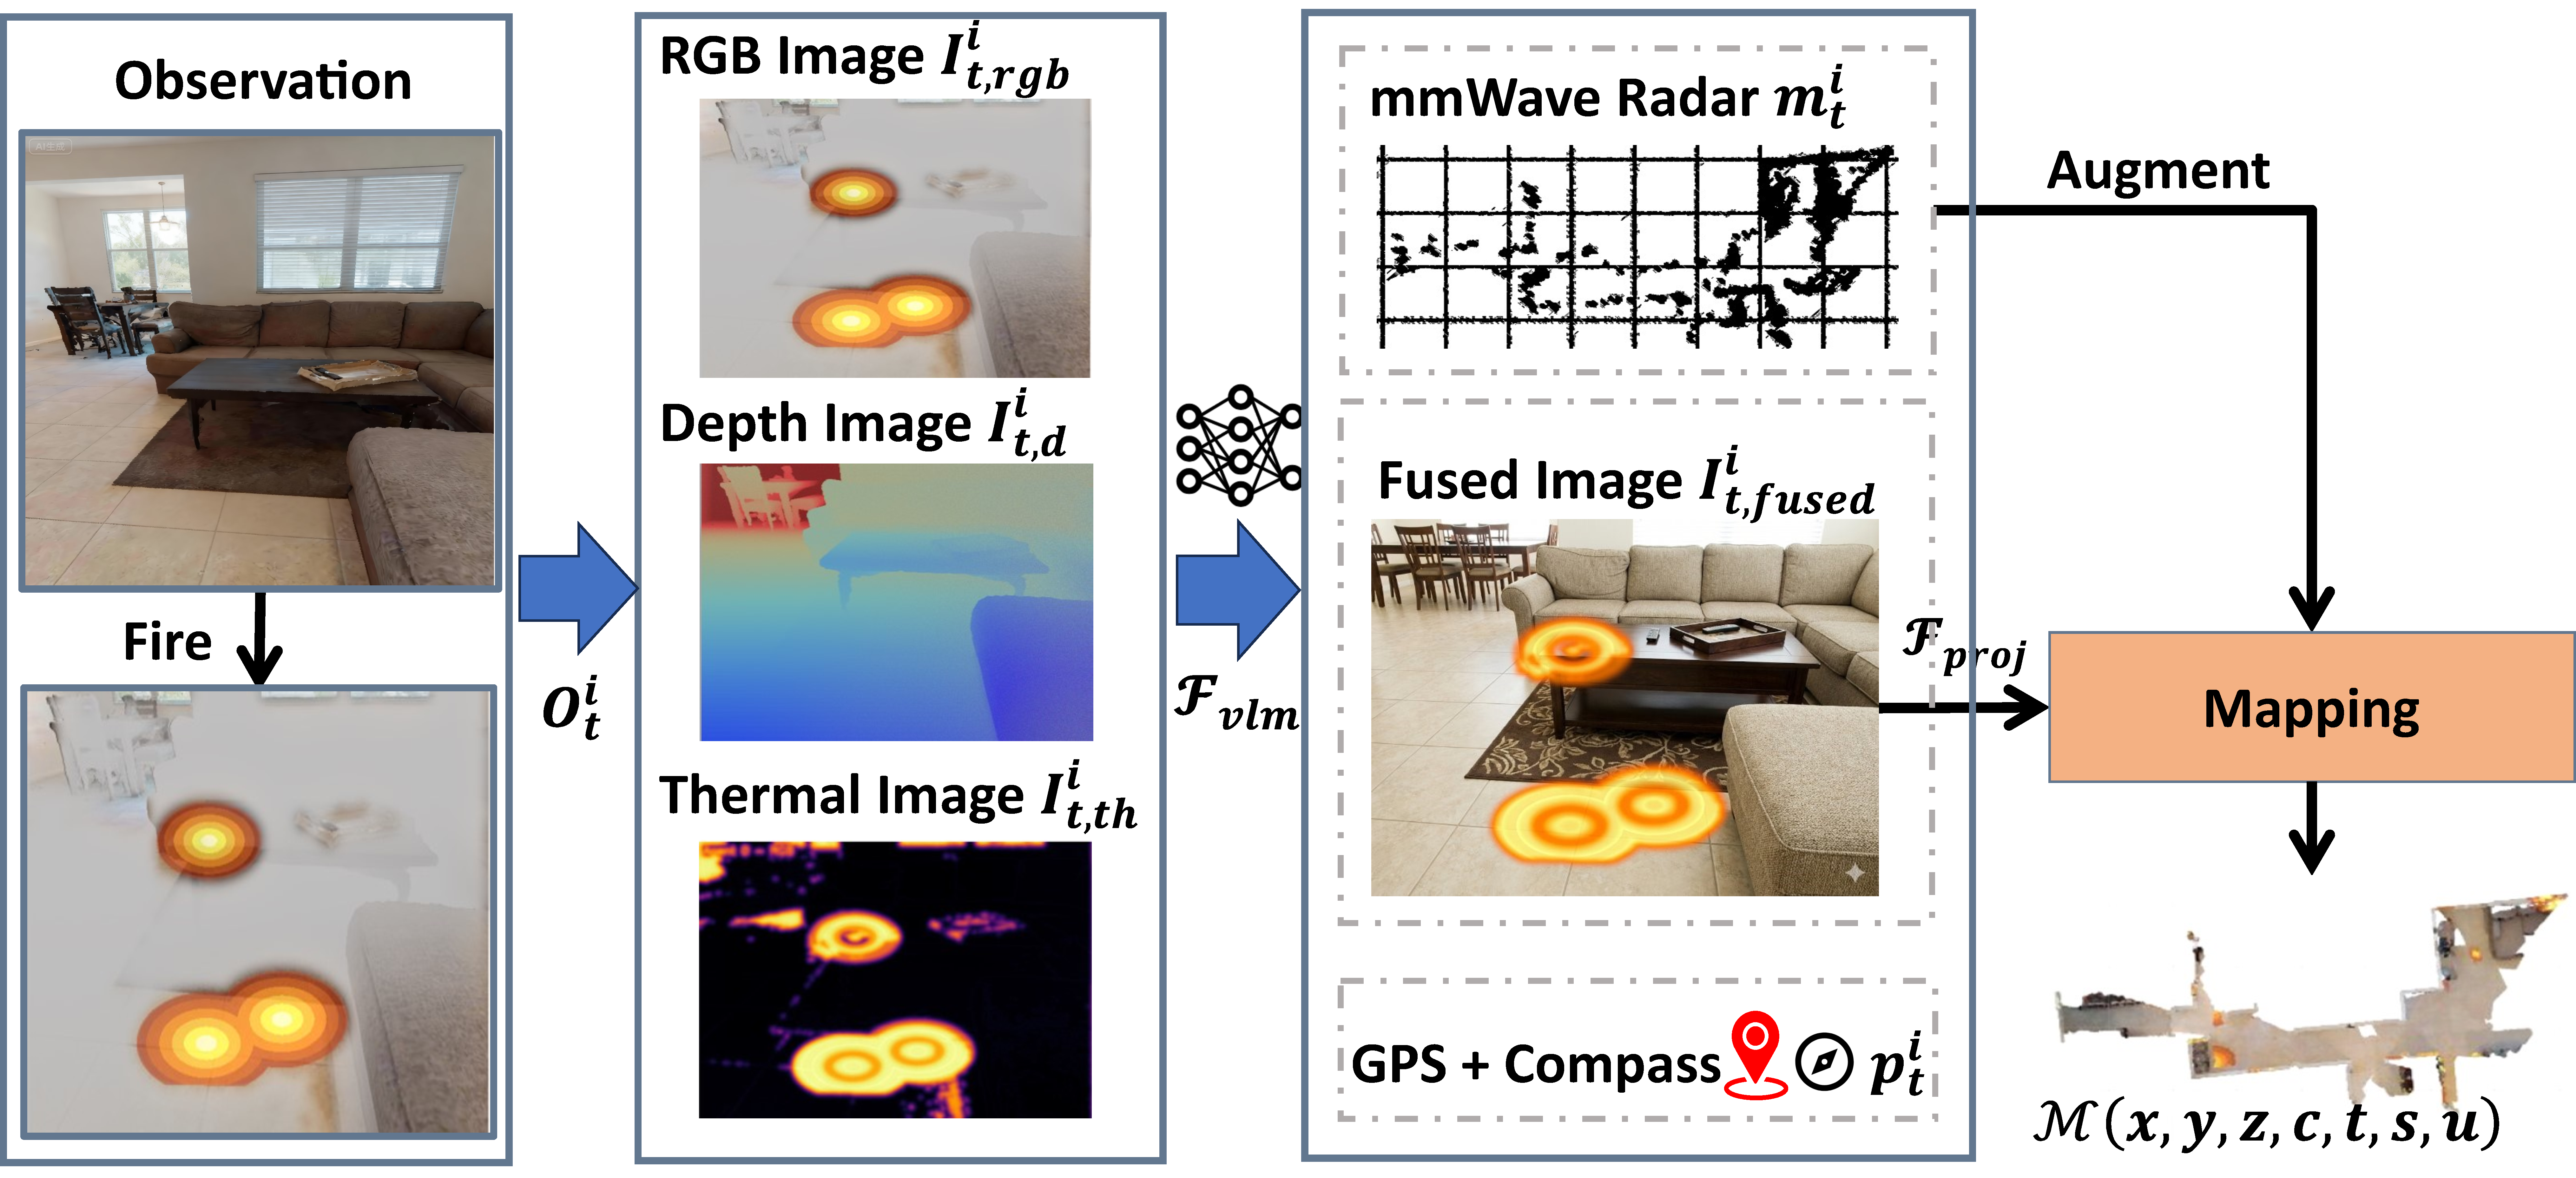
\includegraphics[width=\columnwidth]{figures/multi_modal_perception_and_fusion.pdf}
  \caption{Architecture of multi-modal perception and cross-modal fusion for robust environment understanding.}
  \label{fig:multi_modal_perception_and_fusion}
  \vspace{-15pt}
\end{figure}
% There are some overlaps in the follwing paragraph because there is no change to the detector and segmentation model
An open-vocabulary detector $\mathrm{Det}(\cdot)$ is then applied to the fused image $I^i_{t,\mathrm{fused}}$ to identify candidate objects and fire-related regions. A class-agnostic segmentation model $\mathrm{Seg}(\cdot)$ further extracts pixel-wise masks for these regions. Each pixel $u$ in the fused image, together with its depth $d(u)$, is back-projected to a 3D point in the camera frame: 
\begin{equation}
\mathbf{x}_c(u) = d(u)\mathbf{K}^{-1}\tilde{u},
\end{equation}
where $\mathbf{K}$ is the camera intrinsic matrix and $\tilde{u}$ is the homogeneous pixel coordinate.

Thermal measurements are aligned with RGB pixels to estimate temperature $T(u)$, while smoke density $S(u)$ is inferred from RGB degradation and depth consistency. Each point is augmented with a hazard attribute vector:
\begin{equation}
\mathbf{h} = [T(u), S(u), \sigma(u)],
\end{equation}
where $\sigma(u)$ encodes sensing uncertainty due to occlusion, smoke, or missing depth returns.

The local 3D hazard-aware point cloud is then formed by combining the vision-based points with mmWave radar points:
\begin{equation}
\mathcal{M}_t^{i} =
\mathcal{F}_{\mathrm{proj}} \Big( 
    \mathrm{Seg} \big( \mathrm{Det}(I^i_{t,\mathrm{fused}}) \big) 
\Big) 
\;\cup\; 
m_t^i.
\end{equation}

% Finally, the global hazard-aware 3D point cloud map is constructed by aggregating all robots’ local maps into a common coordinate frame:
% \begin{equation}
% \mathcal{M}^{3D} = \bigcup_{i=1}^{n} \mathcal{F}_{\mathrm{proj}} \big(\mathcal{M}_i^{3D}, p^i_t \big),
% \end{equation}
% where $p^i_t$ is the robot pose at time $t$.
% The local map $\mathcal{M}_i$ is incrementally updated with hazard-aware tuples $(\mathbf{x}_g, \mathbf{h})$ obtained from multi-modal visual perception. In parallel, mmWave radar observations $m_\tau^i$ are used to augment the local map by reinforcing structural occupancy in regions affected by severe visual degradation. 
The global hazard-aware point cloud map $\mathcal{M}$ is then constructed by jointly aggregating vision-based hazard points and mmWave radar points from all robots into a common coordinate frame:
\begin{equation}
\mathcal{M} =
\bigcup_{i=1}^{n}
\;\bigcup_{\tau=1}^{t}
\mathcal{M}_\tau^{i}
\label{eq:global_map}
\end{equation}

To suppress noisy measurements introduced by fire flickering, smoke diffusion, and thermal sensor artifacts, we apply DBSCAN clustering to the merged point cloud and remove sparse outliers.



\subsection{Global Map Construction and Frontier Risk Assessment}
\label{section: Global Map Construction and Frontier Risk Assessment}

To enable efficient risk-aware exploration in fire scenarios, a global 2D obstacle–hazard map is constructed from the 3D point cloud observations collected by the robots. The map provides a compact and physically grounded representation of both structural constraints and environmental hazards.

\subsubsection{2D Obstacle-Hazard Map Construction}

At the beginning of each episode, the global 3D map $\mathcal{M}$ is projected into a 2D grid-based representation centered at the robot's initial position. The resulting map consists of two aligned channels: an obstacle map $\mathbf{O}$ and a hazard map $\mathbf{H}$.

The obstacle map is constructed via top-down projection of non-floor 3D points, where grid cells exceeding a point-density threshold are marked as occupied. This produces a binary occupancy layout used to constrain navigation. The hazard map encodes fire-related environmental risks by aggregating hazard attributes from projected 3D points. Specifically, the hazard intensity of each grid cell is computed as a weighted combination of temperature, smoke density, and sensing uncertainty:
\begin{equation}
\mathbf{H}(x, y) = \sum_{x_g \in (x, y)} \left( w_T T + w_S S + w_\sigma \sigma \right),
\end{equation}
where $w_T$, $w_S$, and $w_\sigma$ balance the contributions of different hazard factors. Together, $\mathbf{O}$ and $\mathbf{H}$ form a compact obstacle–risk abstraction of the fire scene.

\subsubsection{Frontier Extraction and Risk Assessment}

Frontiers are defined as the boundaries between explored and unexplored regions after removing obstacle boundaries from $\mathbf{O}$. Frontier cells are clustered via connected-component analysis, and small noisy clusters are discarded.

Each frontier is assigned a risk score by aggregating hazard intensities within its region. Let $\mathcal{F}_k$ denote the set of grid cells belonging to frontier $k$. The frontier-level risk is defined as:
\begin{equation}
R_k = \frac{1}{|\mathcal{F}_k|} \sum_{(x,y) \in \mathcal{F}_k} \mathbf{H}(x,y).
\end{equation}

Frontiers are then categorized into qualitative risk levels (e.g., safe, moderate, dangerous) using predefined thresholds. Frontiers with lower risk scores are prioritized by the VLM-based planner to enable safe and efficient exploration in fire-disaster environments.



\subsection{GNN-Based Global Planning under Fire Hazards}
\label{subsec:gnn-planner}
After the global map construction and frontier risk assessment, the global planner must, at every replanning tick, assign a long-term frontier goal to each robot in a way that (i) maximizes exploration efficiency by reducing inter-robot redundancy and (ii) minimizes fire exposure by favoring lower-risk frontiers with reliable perception. Recent VLM-based planners~\cite{11302789} address this by querying a remote vision--language model (e.g., GPT-4o) with a top-down map and a structured hazard report. Although the VLM provides strong common-sense priors, each call blocks for ${\sim}20$\,seconds, requires a stable network link, incurs a per-call API cost, and is non-deterministic. In a fire scene this is unacceptable: hazard propagation operates on a tens-of-seconds timescale and the planner itself must be \emph{on-board} and \emph{millisecond-fast}. \system therefore replaces the VLM in the global-planner loop with a small graph neural network (GNN) student distilled from the same VLM via behavior cloning.

\subsubsection{Bipartite Robot--Frontier Graph}
At each replanning step $t$ the planner is given $R$ robots with known poses and $F_t$ candidate frontiers extracted in Sec.~\ref{section: Global Map Construction and Frontier Risk Assessment}, together with their per-frontier risk scores $R_k$. We model the assignment problem as a bipartite graph
\begin{equation}
G_t = (V_R \cup V_{F_t},\, E_t),\quad E_t = V_R \times V_{F_t},
\end{equation}
where $V_R = \{r_1,\dots,r_R\}$ are robot nodes and $V_{F_t} = \{f_1,\dots,f_{F_t}\}$ are frontier nodes. The decision is a per-robot frontier index $y_t^{(r)}\in\{0,\dots,F_t-1\}$. A graph formulation is the natural inductive bias here for three reasons: $F_t$ is small but \emph{varies} per step (a fixed-size MLP would require padding), pairwise robot--frontier relations (relative position, distance, alignment) dominate the decision (an attention mechanism injects them in a permutation-invariant way), and the no-collision coordination constraint (two robots should not select the same frontier) is naturally implemented by stacking robot$\to$frontier and frontier$\to$robot attentions, which produces a competitive signal across the team~\cite{velickovic2018gat}.

The feature builder consumes the existing map outputs of \system and emits three tensors:
\begin{equation}
\begin{aligned}
\mathbf{X}_R &\in \mathbb{R}^{R\times 5}: && [x,\,y,\,\cos\psi,\,\sin\psi,\,F_t], \\
\mathbf{X}_F &\in \mathbb{R}^{F_t\times 5}: && [x,\,y,\,R_k,\,A_k,\,k], \\
\mathbf{E}_{rf} &\in \mathbb{R}^{R\times F_t\times 4}: && [\Delta x,\,\Delta y,\,d_{rf},\,\cos\alpha_{rf}].
\end{aligned}
\end{equation}
All spatial coordinates are normalized by the map size, $R_k$ is the frontier-level hazard score from the hazard map, $A_k$ is the frontier area, $\psi$ is the robot heading, and $\cos\alpha_{rf}$ is the alignment between the robot heading and the line of sight to the frontier (a frontier ahead of the robot is cheaper to reach than one behind it).

\subsubsection{GNN Student Architecture}
The student is a 2-layer cross-attention network with hidden dimension $H=64$ and 4 heads:
\begin{equation}
\small
\begin{aligned}
\tilde{R}^{(\ell)} &= \operatorname{LN}\!\Big(R^{(\ell-1)} + \operatorname{Attn}_{R\to F}(R^{(\ell-1)},F^{(\ell-1)},F^{(\ell-1)};\,\mathbf{E}_{rf})\Big),\\
\tilde{F}^{(\ell)} &= \operatorname{LN}\!\Big(F^{(\ell-1)} + \operatorname{Attn}_{F\to R}(F^{(\ell-1)},\tilde{R}^{(\ell)},\tilde{R}^{(\ell)};\,\mathbf{E}_{rf}^{\!\top})\Big),\\
R^{(\ell)} &= \operatorname{LN}(\tilde{R}^{(\ell)}+\operatorname{MLP}(\tilde{R}^{(\ell)})),\\
F^{(\ell)} &= \operatorname{LN}(\tilde{F}^{(\ell)}+\operatorname{MLP}(\tilde{F}^{(\ell)})).
\end{aligned}
\end{equation}
After $L=2$ layers a small bilinear scoring head produces a logit matrix $\mathbf{S}\in\mathbb{R}^{R\times F_t}$, and at inference we pick $\hat{y}_t^{(r)}=\arg\max_f \mathbf{S}_{r,f}$ per robot, mirroring the structured output of the original VLM prompt. The whole model has fewer than $10^5$ parameters and runs in ${\sim}3$\,ms on a single RTX 4060 Ti, with CPU inference also feasible at ${<}50$\,ms. A safety fallback to a nearest-frontier heuristic is triggered whenever the checkpoint fails to load, so a deployed robot is never left without an action.

\subsubsection{Behavior-Cloning the VLM Teacher}
We frame the imitation problem as supervised classification over frontier indices. The VLM-based planner of \system (the same multi-modal prompt described in prior work~\cite{11302789}, augmented with our per-frontier hazard report) is run once on the training scenes; for each decision step $t$ a non-invasive trace logger records
\begin{equation}
(s_t,\,y_t)=\big(\{\mathbf{X}_R,\mathbf{X}_F,\mathbf{E}_{rf}\}_t,\,\{y_t^{(r)}\}_{r=1}^{R}\big),
\end{equation}
where the labels $y_t^{(r)}$ are parsed from the JSON returned by GPT-4o. Training minimizes a masked cross-entropy with \texttt{ignore\_index}$=-100$ on padded frontiers:
\begin{equation}
\mathcal{L}_{\text{BC}} = -\frac{1}{|B|R}\sum_{(s,y)\in B}\sum_{r=1}^{R}\log\operatorname{softmax}\!\big(\mathbf{S}_r(s)\big)_{y^{(r)}}.
\end{equation}
Trace collection is non-invasive (controlled by a single environment variable), so the existing VLM pipeline is reused unchanged for data collection and is never queried again at deployment time. Optional improvements include distilling soft logits instead of arg-max labels (Hinton-style~\cite{hinton2015distillation}) and iteratively gathering corrective traces in states the student visits but the teacher does not (DAGGER~\cite{ross2011dagger}); we leave both for future work.

\subsubsection{On-Board Frontier Assignment under Fire Hazards}
At deployment time, every $N_g$ local-planning steps ($N_g{=}25$ in our experiments) the GNN receives the updated $(\mathbf{X}_R,\mathbf{X}_F,\mathbf{E}_{rf})$, where $\mathbf{X}_F$ already encodes the per-frontier hazard score $R_k$ from the obstacle--hazard map. The output assignment $\{r_i \!\to\! f_{j}\}$ balances exploration efficiency (the cross-attention block makes the team avoid duplicate goals) and fire safety (frontiers with high $R_k$ are pushed down by the BC objective because the teacher consistently rejected them). If all frontiers exceed a hazard threshold, a fallback policy selects safe waypoints within previously explored low-risk regions. Because the entire global-planning step now costs ${\sim}3$\,ms instead of ${\sim}20$\,s, the planner can re-solve the assignment at every local tick if needed, which is the latency budget that makes truly hazard-reactive multi-robot exploration feasible. The resulting assignment is then passed to the hazard-aware FMM local planner described next.

\subsection{Hazard-Aware Fast Marching Method for Local Planning}

Given the global 2D obstacle and hazard maps, local navigation in fire-driven indoor environments must jointly consider geometric feasibility and environmental risk. We adopt a hazard-aware FMM as the local planner, enabling real-time generation of smooth, collision-free, and risk-sensitive trajectories.

To incorporate fire risk, we modulate the FMM propagation speed using the hazard map:
\begin{equation}
    F(x) = \frac{1}{1 + \alpha H(x)},
\end{equation}
where $H(x)$ encodes aggregated fire-related risk, and $\alpha$ controls the trade-off between safety and efficiency. This formulation penalizes traversal through high-risk regions even when they are geometrically free, while allowing fast propagation in safer areas. 

Applying FMM with the hazard-modulated speed produces an arrival-time field that naturally biases paths toward low-risk corridors. The local trajectory is extracted by following the negative gradient of this field, yielding a smooth path that minimizes accumulated risk while respecting obstacle constraints.


% By grounding local planning on the unified obstacle--hazard map, the proposed hazard-aware FMM provides a reliable execution layer that safely drives agents toward VLM-assigned frontiers under dynamic fire conditions.






